%%%%%%%%%%%%%%%%%%%%%%%%%%%%%%%%%%%%%%%%%
% Journal Article
% LaTeX Template
% Version 1.4 (15/5/16)
%
% This template has been downloaded from:
% http://www.LaTeXTemplates.com
%
% Original author:
% Frits Wenneker (http://www.howtotex.com) with extensive modifications by
% Vel (vel@LaTeXTemplates.com)
%
% License:
% CC BY-NC-SA 3.0 (http://creativecommons.org/licenses/by-nc-sa/3.0/)
%
%%%%%%%%%%%%%%%%%%%%%%%%%%%%%%%%%%%%%%%%%

%----------------------------------------------------------------------------------------
%	PACKAGES AND OTHER DOCUMENT CONFIGURATIONS
%----------------------------------------------------------------------------------------

\documentclass[twoside,twocolumn]{article}

\usepackage{blindtext} % Package to generate dummy text throughout this template 

\usepackage{hyperref}
\hypersetup{
    colorlinks=true,
    linkcolor=blue,
    filecolor=magenta,      
    urlcolor=cyan,
}

\usepackage[sc]{mathpazo} % Use the Palatino font
\usepackage[T1]{fontenc} % Use 8-bit encoding that has 256 glyphs
\linespread{1.05} % Line spacing - Palatino needs more space between lines
\usepackage{microtype} % Slightly tweak font spacing for aesthetics
\usepackage[utf8]{inputenc}

\usepackage[portuguese]{babel} % Language hyphenation and typographical rules

\usepackage[hmarginratio=1:1,top=32mm,columnsep=20pt]{geometry} % Document margins
\usepackage[hang, small,labelfont=bf,up,textfont=it,up]{caption} % Custom captions under/above floats in tables or figures
\usepackage{booktabs} % Horizontal rules in tables

\usepackage{lettrine} % The lettrine is the first enlarged letter at the beginning of the text
\usepackage{float}
\usepackage{enumitem} % Customized lists
\setlist[itemize]{noitemsep} % Make itemize lists more compact

\usepackage{abstract} % Allows abstract customization
\renewcommand{\abstractnamefont}{\normalfont\bfseries} % Set the "Abstract" text to bold
\renewcommand{\abstracttextfont}{\normalfont\small\itshape} % Set the abstract itself to small italic text
%\usepackage[shortlabels]{enumitem}
\usepackage{enumitem}
\usepackage{titlesec} % Allows customization of titles
\renewcommand\thesection{\Roman{section}} % Roman numerals for the sections
\renewcommand\thesubsection{\roman{subsection}} % roman numerals for subsections
\titleformat{\section}[block]{\large\scshape\centering}{\thesection.}{1em}{} % Change the look of the section titles
\titleformat{\subsection}[block]{\large}{\thesubsection.}{1em}{} % Change the look of the section titles

\usepackage{fancyhdr} % Headers and footers
\pagestyle{fancy} % All pages have headers and footers
\fancyhead{} % Blank out the default header
\fancyfoot{} % Blank out the default footer
\fancyhead[C]{MO443 $\bullet$ Abril 2019 $\bullet$ Relatório 01} % Custom header text
\fancyfoot[RO,LE]{\thepage} % Custom footer text

\usepackage{titling} % Customizing the title section

\usepackage{hyperref} % For hyperlinks in the PDF

\usepackage{graphicx}
\usepackage{subfigure}

%----------------------------------------------------------------------------------------
%	TITLE SECTION
%----------------------------------------------------------------------------------------

\setlength{\droptitle}{-4\baselineskip} % Move the title up

\pretitle{\begin{center}\Huge\bfseries} % Article title formatting
\posttitle{\end{center}} % Article title closing formatting
\title{Relatório - Trabalho 01 \\ \Large MO443 - Introdução ao Processamento de Imagem Digital} %
%\subtitle{qsdqwdqwd} %Article title
\author{%
\textsc{Vinicius Teixeira de Melo - RA: 230223} \\[1ex] % Your name
\normalsize Universidade Estadual de Campinas \\ % Your institution
\normalsize \href{mailto:viniciusteixeira@liv.ic.unicamp.br}{viniciusteixeira@liv.ic.unicamp.br} % Your email address
%\and % Uncomment if 2 authors are required, duplicate these 4 lines if more
%\textsc{Jane Smith}\thanks{Corresponding author} \\[1ex] % Second author's name
%\normalsize University of Utah \\ % Second author's institution
%\normalsize \href{mailto:jane@smith.com}{jane@smith.com} % Second author's email address
}
\date{\today} % Leave empty to omit a date
\renewcommand{\maketitlehookd}{%
%\begin{abstract}
%\noindent \blindtext % Dummy abstract text - replace \blindtext with your abstract text
%\end{abstract}
}

%----------------------------------------------------------------------------------------

\begin{document}

% Print the title
\maketitle

%----------------------------------------------------------------------------------------
%	ARTICLE CONTENTS
%----------------------------------------------------------------------------------------

\section{Especificação do Problema}

O objetivo deste trabalho é implementar alguns filtros de imagens no domínio espacial e de frequências. A filtragem aplicada a uma imagem digital é uma operação local que altera os valores de intensidade dos pixels da imagem levando-se em conta tanto o valor do pixel em questão quanto valores de pixels vizinhos.

No processo de filtragem, utiliza-se uma operação de convolução de uma máscara pela imagem. Este processo equivale a percorrer toda a imagem alterando seus valores conforme os pesos da máscara e as intensidades da imagem.

O trabalho está dividido em duas seções principais:

\begin{itemize}
	\item Filtragem no Domínio Espacial
	\item Filtragem no Domínio de Frequências
\end{itemize}

Na seção de filtragem no domínio espacial, são dados 4 seguintes tipos de filtros:

\begin{enumerate}[label=(\alph*)]
\item $h_{1} = $ \begin{tabular}[H]{|c|c|c|c|c|}
\hline
0  & 0  & -1 & 0  & 0  \\ \hline
0  & -1 & -2 & -1 & 0  \\ \hline
-1 & -2 & 16 & -2 & -1 \\ \hline
0  & -1 & -2 & -1 & 0  \\ \hline
0  & 0  & -1 & 0  & 0  \\ \hline
\end{tabular}

\item $h_{2} = \frac{1}{256}$ \begin{tabular}{|c|c|c|c|c|}
\hline
1 & 4  & 6  & 4  & 1 \\ \hline
4 & 16 & 24 & 16 & 4 \\ \hline
6 & 24 & 36 & 24 & 6 \\ \hline
4 & 16 & 24 & 16 & 4 \\ \hline
1 & 4  & 6  & 4  & 1 \\ \hline
\end{tabular}

\item $h_{3} = $ \begin{tabular}{|c|c|c|}
\hline
-1 & 0 & 1 \\ \hline
-2 & 0 & 2 \\ \hline
-1 & 0 & 1 \\ \hline
\end{tabular}

\item $h_{4} = $ \begin{tabular}{|c|c|c|}
\hline
-1 & -2 & -1 \\ \hline
0  & 0  & 0  \\ \hline
1  & 2  & 1  \\ \hline
\end{tabular}
\end{enumerate}

As aplicações dos filtros devem ser feitas de forma individual, porém, os filtros $h_{3}$ e $h_{4}$ devem ser aplicados de forma combinada, somando-se as respostas de cada um dos filtros por meio da seguinte expressão: $\sqrt{(h_{3})^{2} + (h_{4}})^{2}$.

Na seção de filtragem no domínio de frequências, é necessário aplicar um filtro Gaussiano em uma imagem representada por seu espectro de Fourier, e a componente de frequência zero deve ser transladada para o centro do espectro. Nesse experimento, é necessário testar diferentes graus de suavização, de formaa borrar a imagem com mais ou menos intensidade.

%------------------------------------------------

\section{Entrada de Dados}

O código fonte criado para a execução de todas as tarefas está no notebook \textbf{Trabalho 01.ipynb}. O código foi criado para aceitar imagens em tons de cinza no formato RGB (\textit{Red, Green and Blue}) do tipo PNG (\textit{Portable Network Graphics}).

Para executar o notebook, basta iniciar o ambiente \textit{Jupyter Notebook}, abrir o notebook \textbf{Trabalho 01.ipynb} e executar as células em ordem. Todo o algoritmo foi implementado na linguagem Python na versão 3.6.

As imagens de entrada utilizadas nos testes do algoritmo foram retiradas da página do prof. Hélio Pedrini: \href{http://www.ic.unicamp.br/~helio/imagens_png/}{Imagens}. Na pasta \textbf{imgs/} estão as duas imagens monocromáticas utilizadas nos testes: \textbf{baboon.png} e \textbf{butterfly.png}. As dimensões das imagens de entrada utilizadas são 512x512.

\begin{figure}[tb]
\begin{center}
	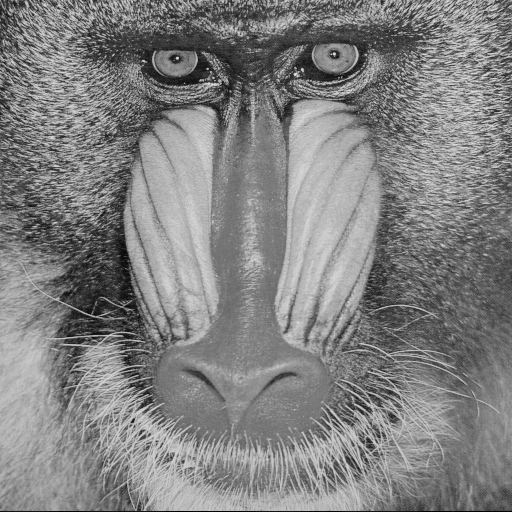
\includegraphics[height=5cm]{figures/baboon.png}
\caption{baboon.png} \label{gdimotes}
\end{center}
\end{figure}

\begin{figure}[tb]
\begin{center}
	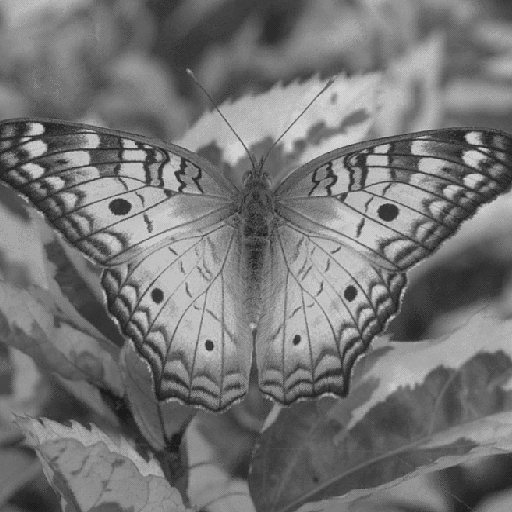
\includegraphics[height=5cm]{figures/butterfly.png}
\caption{butterfly.png} \label{gdimotes}
\end{center}
\end{figure}

%------------------------------------------------

\section{Código e Decisões Tomadas}

\subsection{Preenchimento de borda}

\subsection{Convolução 2D}

\subsection{Redimensionamento}


%------------------------------------------------

\section{Saída de Dados}

%------------------------------------------------

\section{Resultados}

%----------------------------------------------------------------------------------------
%	REFERENCE LIST
%----------------------------------------------------------------------------------------

\begin{thebibliography}{99} % Bibliography - this is intentionally simple in this template

\bibitem[Figueredo and Wolf, 2009]{Figueredo:2009dg}
Figueredo, A.~J. and Wolf, P. S.~A. (2009).
\newblock Assortative pairing and life history strategy - a cross-cultural
  study.
\newblock {\em Human Nature}, 20:317--330.
 
\end{thebibliography}

%----------------------------------------------------------------------------------------

\end{document}
